\section{Stattegger Straße Nord}
Die \index{Stattegger Straße} stellt im Norden von Andritz eine wichtige Verbindung in die Stadt dar. Sowohl der nördliche Teil von Andritz als auch fast der gesamte Bezirk Stattegg sind auf diese Straße als Hauptverbindungsroute angewiesen.

Aktuell ist die Stattegger Straße für Radfahrer und Fußgänger jedoch relativ ungeeignet, das Potential zur Förderung des sanften Verkehrs jedoch sehr hoch.

\subsection{Status Quo}
% TODO: Beschreibung des Verlaufs der Stattegger Straße mit Fotos

Die Grenze zwischen Graz und Stattegg liegt bei der Adresse Stattegger Straße 143. Dennoch sollte eine Radinfrastruktur hier möglichst durchgängig geplant und zusammen mit der Gemeinde Stattegg geplant und umgesetzt werden.

\subsubsection{Fuß der Leber bis Hub}
Am nördlichen Ende geht die Stattegger Straße bei der Pension \index{Statteggerwirt} in die \index{Leberstraße} über. Die Leberstraße ist schmal und sehr steil und führ zu einem relativ kleinen Einzugsgebiet, das oft über andere Routen besser angeschlossen werden könnte.

\begin{wrapfigure}{L}{0.7\textwidth}
\centering
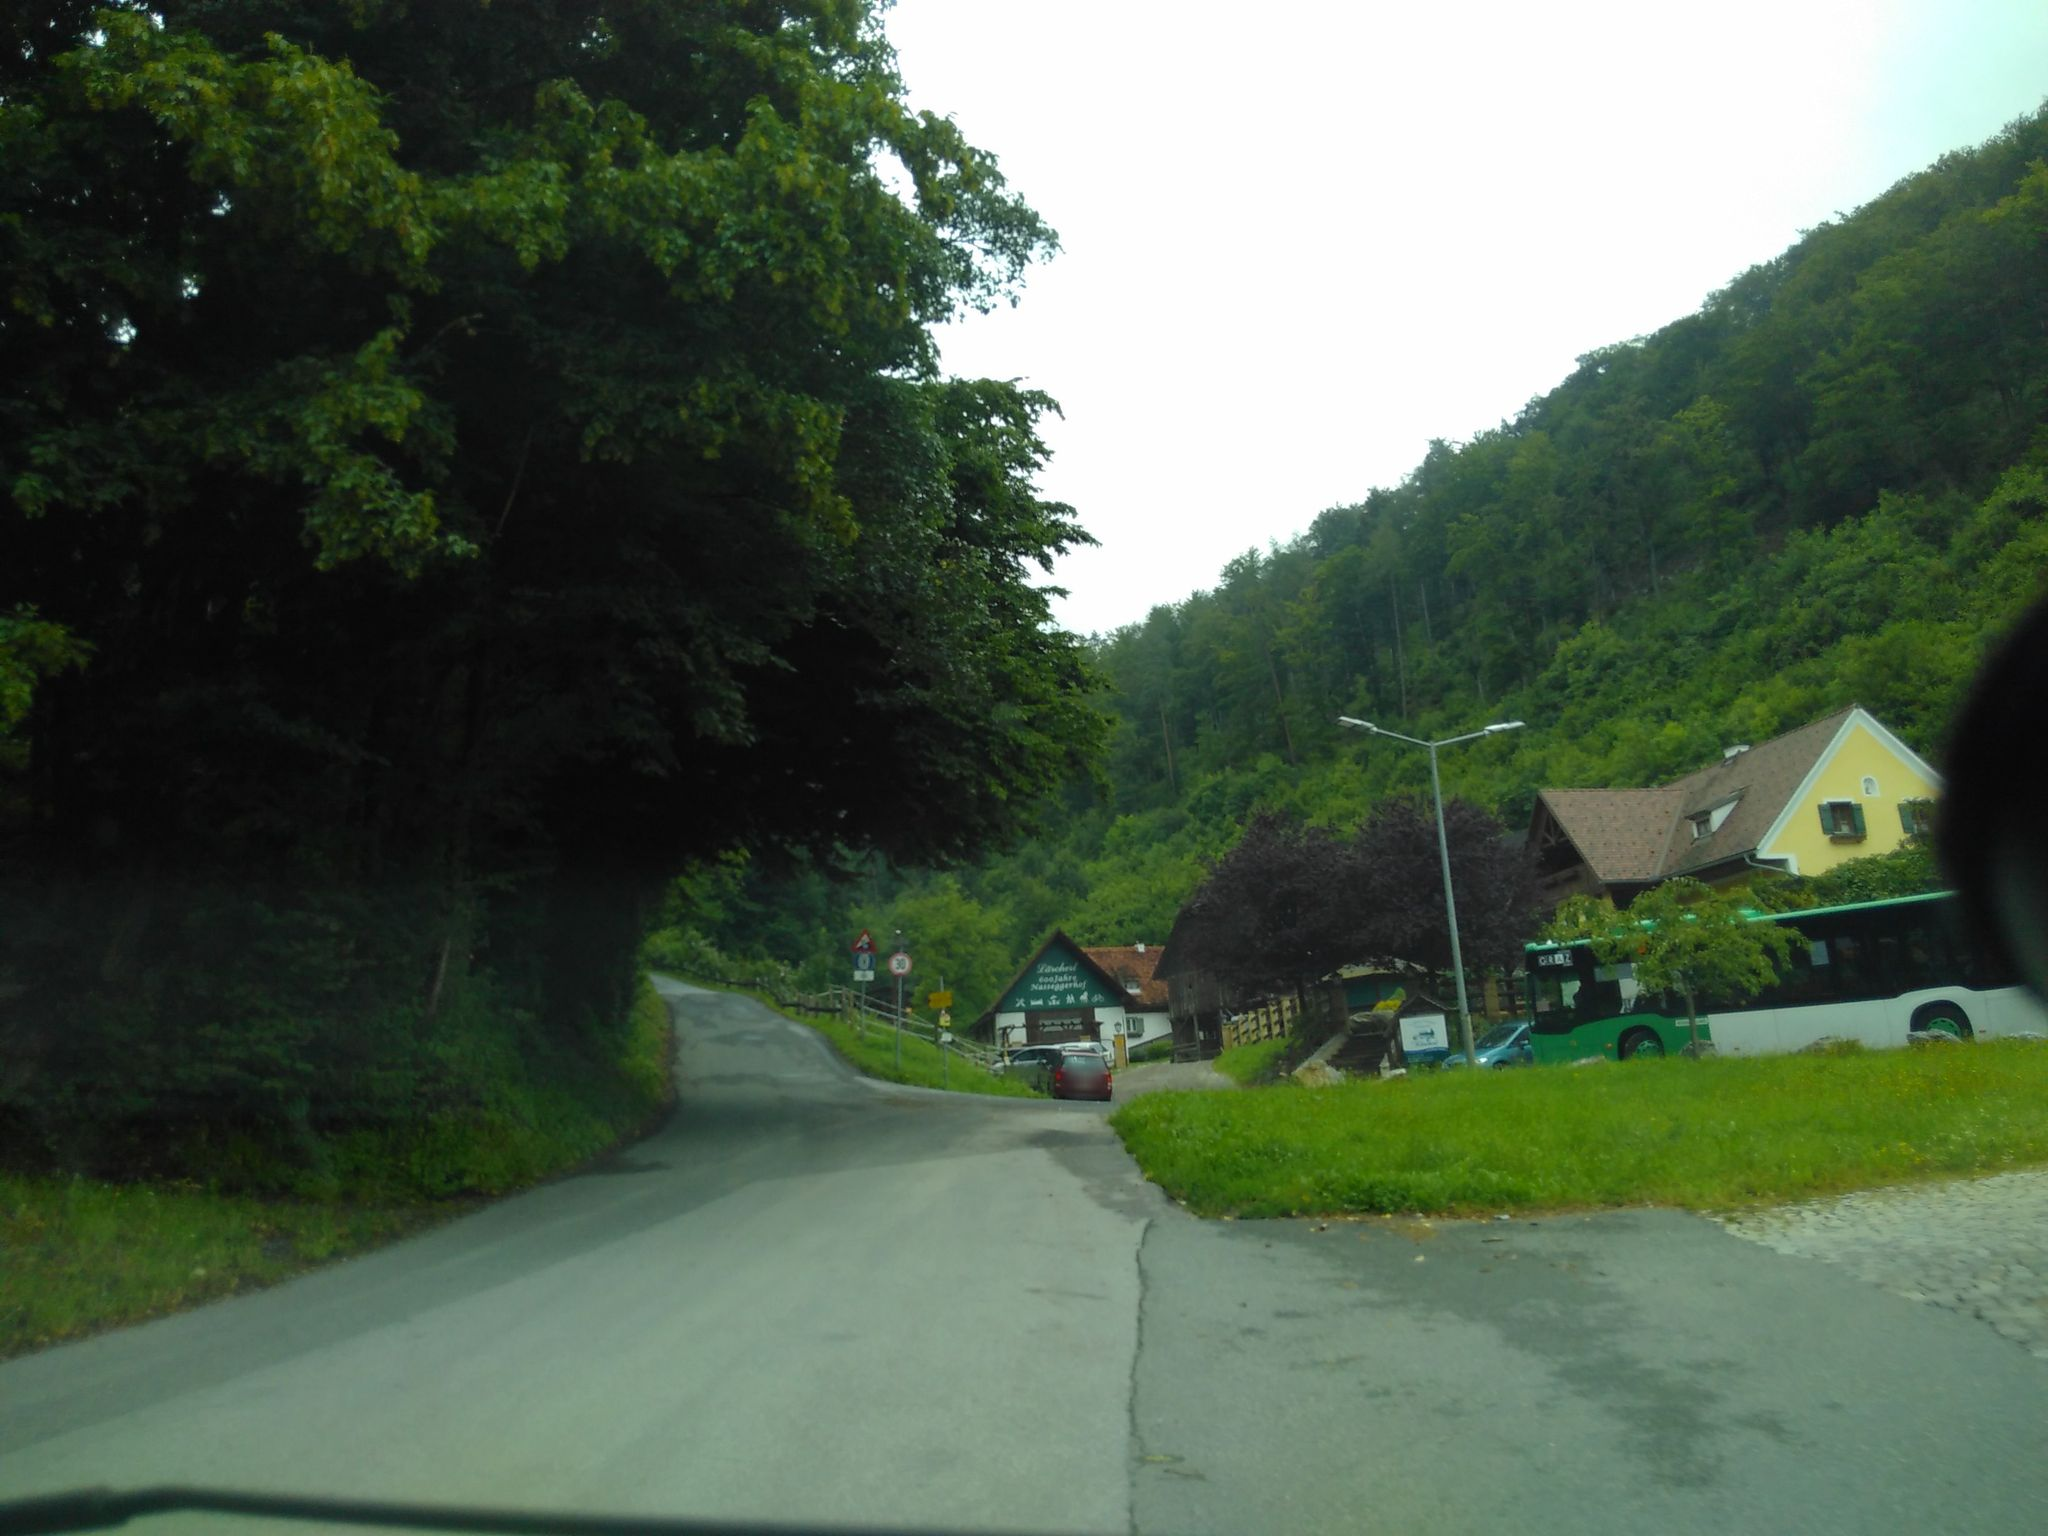
\includegraphics[width=0.7\textwidth]{main/bike/andritz/stattegger_straße_nord/statteggerwirt}
\caption[Pension Statteggerwirt]{Pension Statteggerwirt und erstes Stück der Leberstraße von Süden. Foto von tobiaso.}
\end{wrapfigure}

Bei der Pension Statteggerwirt befindet sich außerdem die Endstation der \index{Buslinie!53}Buslinie 53, die von hier im Viertelstundentakt über den Andritzer Hauptplatz zum Hauptbahnhof führt. 

\subsection{Vision}
